Consider the problem of checking if a set of nodes $S$ in a graph $G$ is
reachable from an arbitrary node $N$. An obvious solution to this problem is to
start at $N$, gather all the neighbor nodes into a list and then recursively
visit all those reachable nodes, until $S$ is covered. This reduces to a problem
of performing a breadth or depth-first search on graph $G$. However, this
solution is sequential and does not have much concurrency.  An alternative
solution to the problem is to recursively propagate the search to all neighbors
and aggregate the results in the node where the search started.  The code for
this later solution is shown in Fig.~\ref{code:threads:reach_simple}.

\begin{figure}[h]
\begin{Verbatim}[numbers=left,fontsize=\codesize,commandchars=*\#\&]
type int id.*hfill// Type declaration
type list int reach-list.

type edge(node, node).*hfill// Predicate declaration
type value(node, int).
type linear search(node, id, reach-list).
type linear do-search(node, id, node, reach-list).
type linear lookup(node, id, reach-list, int Val).
type linear new-lookup(node, id, int Val).
type linear visited(node, id).

search(A, Id, ToReach)*label#line:threads:reach_lookup1&*hfill// Rule 1: initialize search
   -o do-search(A, Id, A, ToReach),
      lookup(A, Id, ToReach, []).*label#line:threads:reach_lookup2&

lookup(A, Id, ToReach, Found), new-lookup(A, Id, Val)*hfill// Rule 2: new reachable node found
   -o lookup(A, Id, remove(ToReach, Val), [Val | Found]).

do-search(A, Id, Node, ToReach),*label#line:threads:reach_visit1&*hfill// Rule 3: node has already seen this search
visited(A, Id)
   -o visited(A, Id). *label#line:threads:reach_visit2&

do-search(A, Id, Node, ToReach),*hfill// Rule 4: node found and propagate search
!value(A, Val), Val in ToReach*hfill// New node was found.
   -o visited(A, Id),*label#line:threads:reach_visit_visited1&
      new-lookup(Node, Id, Val),
      {B | !edge(A, B) -o do-search(B, Id, Node, remove(ToReach, Val))}.*label#line:threads:reach_propagate&

do-search(A, Id, Node, ToReach),*hfill// Rule 5: node not found and propagate search
!value(A, Val), ~ Val in ToReach*hfill// Not the node we are looking for.
   -o {B | !edge(A, B) -o do-search(B, ID, Node, ToReach)},*label#line:threads:reach_propagate2&
      visited(A, Id).*label#line:threads:reach_visit_visited2&
\end{Verbatim}

\caption{LM code to perform reachability checking on a graph.}
\label{code:threads:reach_simple}
\end{figure}

Each distinct reachability search is represented by a number (\code{Id}) and a
\code{search} axiom. Associated to each search \code{Id} is a list of nodes to
reach.  The predicate \code{visited} marks nodes that have already
participated in search, while predicate \code{do-search} is used to propagate a
specific search. The first rule
(lines~\ref{line:threads:reach_lookup1}-\ref{line:threads:reach_lookup2}) starts
a particular search by deriving a \code{do-search} and an \code{lookup} fact.
The \code{lookup} fact is used as an accumulator and is stored in the starting
node. The third rule
(lines~\ref{line:threads:reach_visit1}-\ref{line:threads:reach_visit2}) avoids
visiting the same node twice in the presence of a \code{visited} fact.  This
visited fact is derived in the next two rules
(lines~\ref{line:threads:reach_visit_visited1}
and~\ref{line:threads:reach_visit_visited2}).  If the node where the search is
being performed is in the set of nodes we want to reach (\code{ToReach}) then we
remove the node value from the list and propagate the search to the neighbor
nodes (line~\ref{line:threads:reach_propagate}).  Otherwise, the search is
propagated but no value is removed from \code{ToReach}.

As an example, consider Fig.~\ref{fig:threads:reach_example}, which shows 2
reachability checks on a graph with 10 nodes. For instance, the search with
\code{Id = 0} starts at node \code{@1} and checks if nodes \code{@1}, \code{@2},
and \code{@3} are reachable from \code{@1}. Since \code{@1} is the starting
node, \code{1} is immediately removed from the reachable list, including the
propagated \code{do-search} facts but also the \code{lookup} fact that is stored
at node \code{@1}. Once \code{do-search} reaches node \code{@3}, the value
\code{3} is removed from the list and a new \code{do-search} is propagated to
node \code{@1} (not shown in the figure) and \code{@2}. At the same time, node
\code{@2} receives the list \code{[2,3]}, removes \code{2} and propagates
\code{[3]} to node \code{@3} and \code{@1}. Node \code{@1} receives two
\code{new-lookup} facts, one from \code{@3} and another from \code{@2}, due to
successful searches and the \code{lookup} fact becomes \code{lookup(@1,0,[],
[1,2,3])}.

The attentive reader will notice that node \code{@1} already knows that all the
nodes have been reached and that nodes \code{@7} and \code{@4} will, needlessly,
continue to check if \code{[2,3]} are reachable. This is an issue that arises
because the programmer has valued concurrency by increasing redundancy and
reducing communication between nodes. It would be prohibitly expensive to share
reachability information between nodes. An alternative solution is to store the
results of the search on the thread performing the search and then coordinate
the results with other threads since the number of threads is usually smaller
than the number of nodes. Before showing how the reachability program is solved
using thread-based facts, we first present the changes to the language.

\begin{figure}[ht]
\begin{center}
   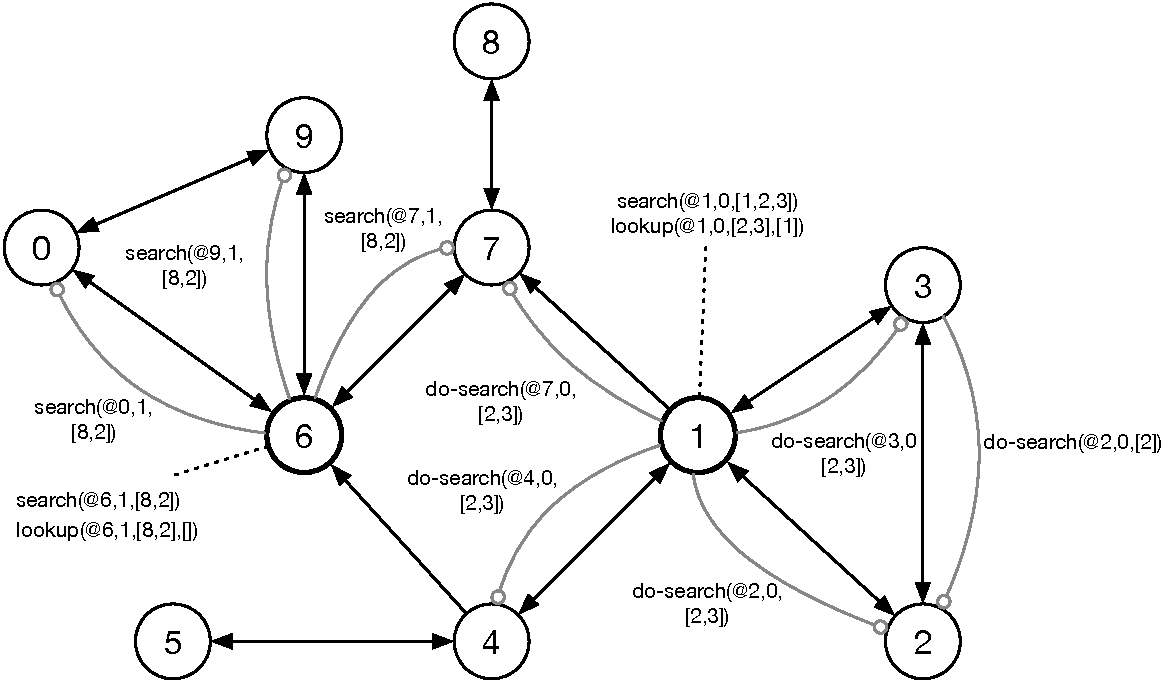
\includegraphics[width=0.9\linewidth]{figures/threads/reach.pdf}
\end{center}

\caption{Performing reachability checks on a graph using nodes \code{@1}
(\code{Id = 0}) and \code{@6} (\code{Id = 1}).  Search with \code{Id = 0} wants
to reach nodes \code{@1}, \code{@2}, and \code{@3} from node \code{@1}. Since
\code{@1} is part of the target nodes, the fact \code{do-search} propagated to
neighbor nodes does not include \code{1}.}

\label{fig:threads:reach_example}
\end{figure}

\subsection{Language Changes}

In the previous chapter, we presented coordination facts such as
\code{thread-id} and \code{set-thread} that already bring some awareness about
the underlying parallel system. Furthermore, such facts also introduce the
\code{thread} type for predicate arguments, which refers to a thread in the
system that is related to a core in a multi core processor. We now introduce the
concept of \emph{thread facts}, which are logical facts stored at the thread
level, meaning that, each thread is now an entity with its own logical facts.
The type \code{thread} is also now the type of the first argument of
\emph{thread predicates}, indicating that the predicate is related and is to be
stored in a specific thread. We also view the available threads as forming a
separate graph from the data graph, a graph of the processing units which are
operating on the data graph.

The introduction of thread facts increases the expressiveness of the system in
the sense that it is now possible to write inference rules that reason about the
state of the threads. This creates optimization opportunies since we can now
write algorithms with global information stored in the thread, while keeping the
LM language fully declarative. Moreover, threads are now allowed to explicitly
communicate with each other, and in conjunction with coordination predicates,
enable the writing of complex scheduling policies.

We discriminate between two new types of inference rules. The first type is the
\emph{thread rule} and has the form \code{a(T), b(T) -o c(T)}, and can be read
as: if thread \code{T} has fact \code{a(T)} and \code{b(T)} then derive fact
\code{c(T)}. The second type is the \emph{mixed rule} and has the form
\code{a(T), d(N) -o e(N)} and can be read as: if thread \code{T} is executing
node \code{N} and has the fact \code{a(T)} and node \code{N} has the fact
\code{d(N)} then derive \code{e(N)} at node \code{N}. Thread rules reason solely
at the thread level, while mixed rules allow reasoning about both thread and
node facts. Logically, the mixed rule uses an extra fact \code{running(T, N)},
which indicates that thread \code{T} is currently executing node \code{N}. The
\code{running} fact is implicitly retracted and asserted every time the thread
selects a different node for execution. This makes our implementation efficient
since a thread does not need to look for nodes that match mixed rules and it is
then the scheduling of the program that drives the matching of such rules.

\subsection{Graph Of Threads}

Figure~\ref{fig:coord:thread_facts} represents a schematic view of the two graph
data structures of a program with three threads: thread $T1$ is executing node
\code{@5}, $T2$ is executing node \code{@4}, and $T3$ is executing node
\code{@3}. Note that every thread has access to its own facts and to the node
facts.

\begin{figure}[ht]
   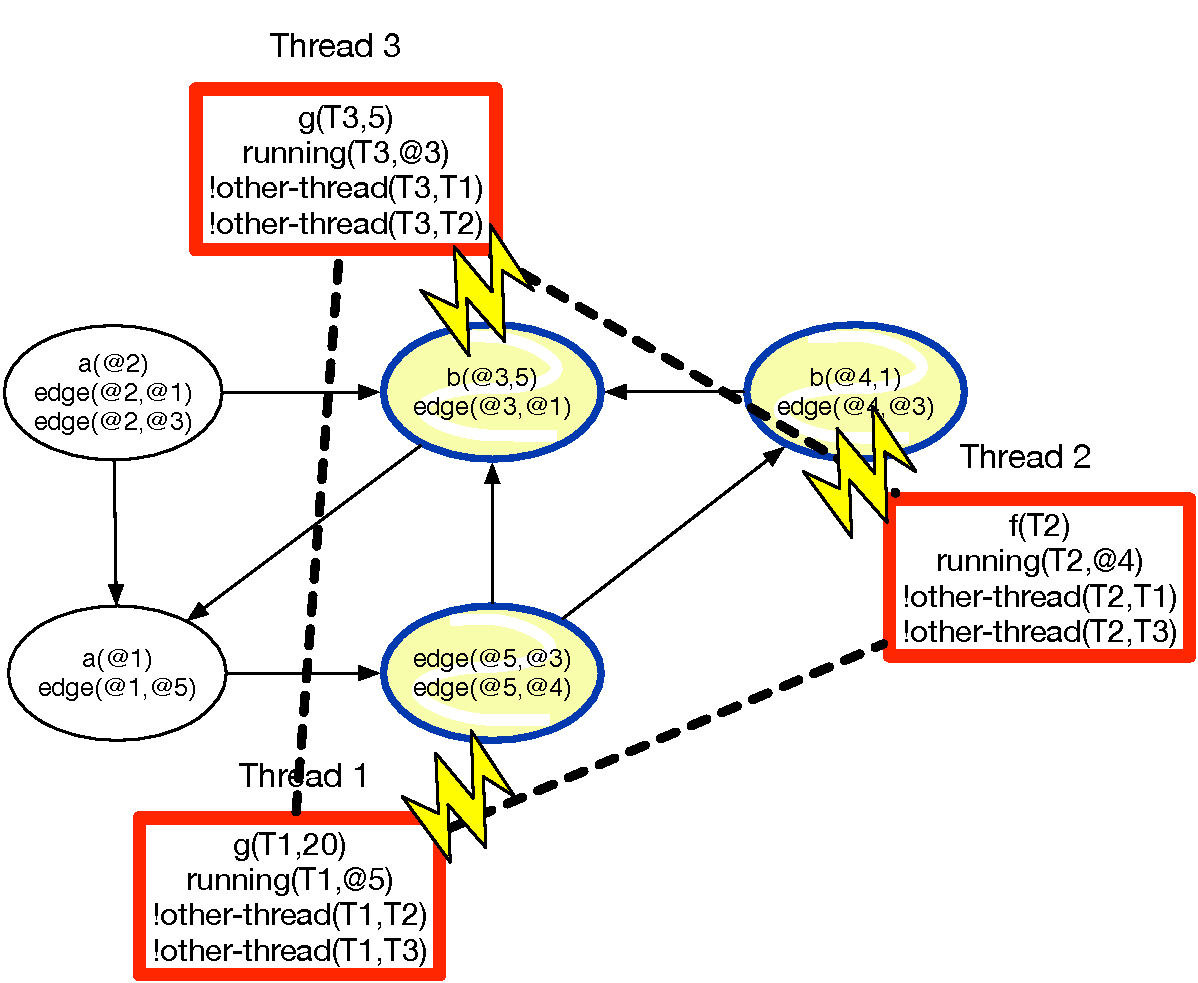
\includegraphics[width=0.6\linewidth]{figures/threads/threads.pdf}

   \caption{An example program being executed with three threads. Note that each
      threads has a \code{running} fact that stores the node currently being
   executed.}

   \label{fig:coord:thread_facts}
\end{figure}

We added several helpful predicates that allow the programmer to inspect the
graph of threads and reason about the state of computation as it relates to
threads:

\begin{itemize}
   \item \code{\bang thread-list(T, L)}: Fact instantiated in all threads where
      \code{L} is a list of all threads executing in the system.

   \item \code{\bang other-thread(T1, T2)}: Connects thread \code{T1} to all the
      other threads \code{T2} executing in the system. Note that in
      Fig.~\ref{fig:coord:thread_facts}, we use \code{\bang other-thread} fact
      to specify the graph of threads.


   \item \code{\bang leader-thread(T, TLeader)}: Fact instantiated in all
      threads where \code{TLeader} refers to a selected thread (the first thread
      in \code{L} of \code{\bang thread-list(T, L)}).

   \item \code{running(T, A)}: Used to retrieve the current node \code{A}
      running on thread \code{T}.
\end{itemize}

With the exception of \code{running}, every other fact is added at the beginning
of the program as a persistent fact.

\subsection{Reachability With Thread Facts}

We know update the graph reachability program presented in
Fig.~\ref{code:threads:reach_simple} to use thread facts in order to avoid
needless searches on the graph. The search process is still done concurrently as
before, but the search state is now stored in each thread, allowing the thread
to store partial results and coordinate with other threads. The code for this new
version is shown in Fig.~\ref{code:threads:reach_threads}.

Lines~\ref{line:threads:reacht_start1}-\ref{line:threads:reacht_start2} start
the search process by assigning a thread \code{Owner} to search \code{Id} using
the persistent fact \code{\bang thread-list} which contains the list of all
available threads in the system. Next, in
line~\ref{line:threads:reacht_threads}, a fact \code{thread-search} is created
for all threads using a comprehension. We use predicate \code{do-search} to
propagate the search through the graph and a predicate \code{visited} to mark
nodes already processed for a specific search.  The two rules in
lines~\ref{line:threads:reacht_check1}-\ref{line:threads:reacht_check2}
propagate the search process to the neighbor nodes and check if the current node
is part of the list of nodes we want to reach.

An interesting property of this version is that each owner thread responsible
for a search keeps track of the remaining nodes that need to be reached. In
line~\ref{line:threads:reacht_remove}, we derive \code{remove-thread-search} in
order to inform owner threads about new reachable nodes. Once an owner thread
detects that all nodes have been reached (lines
\ref{line:threads:reacht_reached1}-\ref{line:threads:reacht_reached2}), all the
other threads will know that and update their search state accordingly
(lines~\ref{line:threads:reacht_knows1}-\ref{line:threads:reacht_knows2}). When
every thread knows that all nodes were reached, they will consume
\code{do-search} facts (lines
\ref{line:threads:reacht_prune1}-\ref{line:threads:reacht_prune2}), effectively
pruning the search space.

\begin{figure}[h]
\begin{Verbatim}[numbers=left,fontsize=\codesize,commandchars=*\#\&]
search(A, Id, ToReach),*label#line:threads:reacht_start1&*hfill// Rule 1: initialize search
*textbf#!thread-list(T, L)&, Owner = nth(L, Id % @threads)*hfill// Allocate search to a thread
   -o {T2 | *textbf#!other-thread(T, T2)& -o *textbf#thread-search(T2, Id, ToReach, Owner)&},*label#line:threads:reacht_threads&
      do-search(A, Id).*label#line:threads:reacht_start2&

*textbf#thread-search(T, Id, [], Owner)&, *label#line:threads:reacht_prune1&*hfill// Rule 2: search completed
do-search(A, Id)
   -o *textbf#thread-search(T, Id, [], Owner)&. *label#line:threads:reacht_prune2&

do-search(A, Id),*hfill// Rule 3: node already visited
visited(A, Id)
   -o visited(A, Id).

do-search(A, Id),*label#line:threads:reacht_check1&*label#line:bfs_join1&*hfill// Rule 4: node found
*textbf#thread-search(T, Id, ToReach, Owner)&,*label#line:threads:reacht_join2&
!value(A, Val), Val in ToReach
   -o *textbf#thread-search(T, Id, remove(ToReach, Val), Owner)&,
      *textbf#remove-thread-search(Owner, Id, Val)&,*hfill// Tell owner thread about it.*label#line:threads:reacht_remove&
      {B | !edge(A, B) -o do-search(B, Id)},
      visited(A, Id).

do-search(A, Id),*hfill// Rule 5: node not found but propagate search
*textbf#thread-search(T, Id, ToReach, Owner)&,
!value(A, Val), ~ Val in ToReach
   -o *textbf#thread-search(T, Id, ToReach, Owner)&,
      visited(A, Id),
      {B | !edge(A, B) -o do-search(B, Id)}.*label#line:threads:reacht_check2&

*textbf#remove-thread-search(T, Id, Val), thread-search(T, Id, ToReach, Owner)&*hfill// Rule 6: node found
   *textbf#-o thread-search(T, Id, remove(ToReach, Val), Owner),&
      *textbf#check-results(T, Id).&

*textbf#check-results(T, Id),&*label#line:threads:reacht_reached1&*hfill// Rule 7: search is completed
*textbf#thread-search(T, Id, [], Owner)&
   *textbf#-o thread-search(A, Id, [], Owner),&
      *textbf#{B | !other-thread(T, B) -o signal-thread(B, Id)}.&*label#line:threads:reacht_reached2&

 *textbf#check-results(T, Id),&*hfill// Rule 8: search not completed yet
 *textbf#thread-search(T, Id, ToReach, Owner), ToReach <> []&
   *textbf#-o thread-search(T, Id, ToReach, Owner).&

*textbf#signal-thread(T, Id),&*hfill// Rule 9: thread knows search is done*label#line:threads:reacht_knows1&
*textbf#thread-search(T, Id, ToReach, Owner)&
   *textbf#-o thread-search(T, Id, [], Owner).& *label#line:threads:reacht_knows2&
\end{Verbatim}
\caption{Coordinated version of the reachability checking program. Note
that \code{@threads} represent the number of threads in the system.}
\label{code:threads:reach_threads}
\end{figure}

An alternative implementation could force every thread to share its reached
nodes to all the other threads in the system. However, this would generate a lot
of traffic between threads, which would actually make the program perform worse.
Our final solution is a good trade off since it only forces threads to
coordinate when pruning can actually happen.

Figure~\ref{fig:threads:results_search} presents experimental results of the
graph reachability program using 4 different datasets. Except for Random, all
the datasets were already used in the MSSD program and were presented before.
The Random dataset is a randomly generated graph with 50000 nodes and about a
million edges.  In the plots, we show the run time of the version without thread
facts (\textbf{Regular}) and the version using thread facts called
\textbf{Threads}. We also show the speedup of the \textbf{Threads} and
\textbf{Regular} versions against the \textbf{Regular} version with 1 thread.

Our results indicate that using thread facts produces a significant reduction in
run time. This is especially true in the case of datasets with large number of
edges, since less facts are produced and propagated in the graph when the
threads know that the search has been completed. The results also show that, in
the case of the Facebook dataset, in which the number of queries is the same as
the number of nodes, the use of thread facts does not produce great improvements
due to the costs of managing the reachability results on each thread's database.
These costs are related to the need to index and lookup \code{thread-search}
facts on the \code{Id} argument every time a node is inspected.

\begin{figure}[]
        \centering
        \begin{subfigure}[b]{\plotsize\textwidth}
           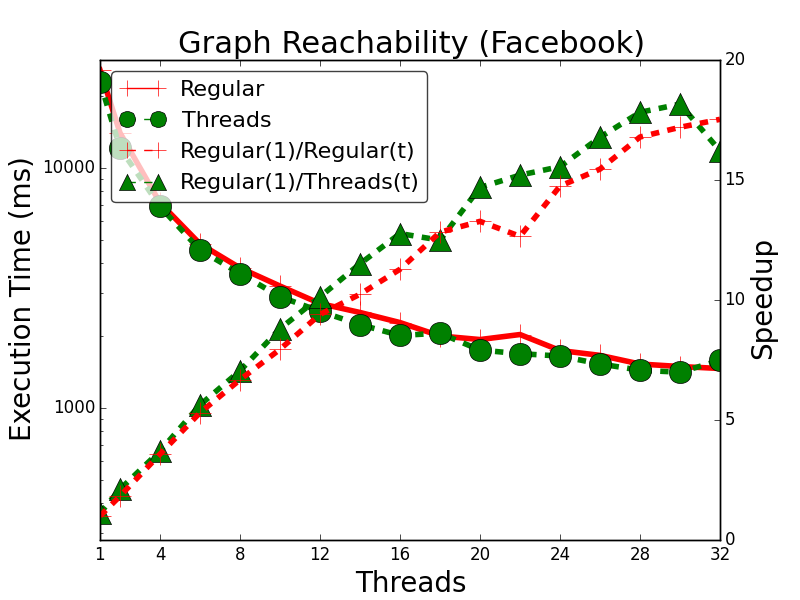
\includegraphics[width=\textwidth]{experiments/threads/cmp-search-facebook.png}
           \caption{Facebook has 2000 nodes and 20000 edges. The dataset makes
           2000 graph queries to 5\% of the graph's nodes.}
           \label{fig:threads:search_facebook}
        \end{subfigure}
        \spacing
        \begin{subfigure}[b]{\plotsize\textwidth}
           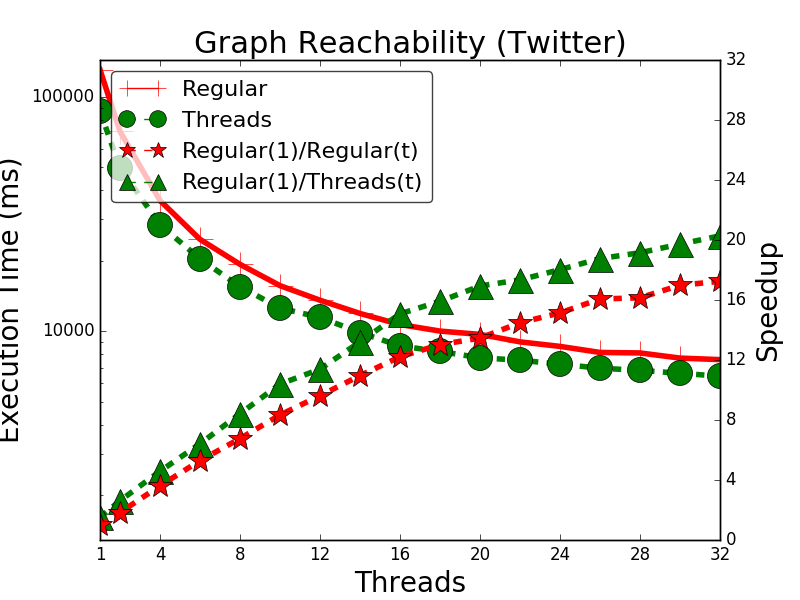
\includegraphics[width=\textwidth]{experiments/threads/cmp-search-twitter.png}
           \caption{Twitter has 81306 nodes and 1768149 edges. The dataset makes
           100 graph queries to 1\% of the graph's nodes.}
           \label{fig:threads:search_twitter}
        \end{subfigure} \\
        \begin{subfigure}[b]{\plotsize\textwidth}
           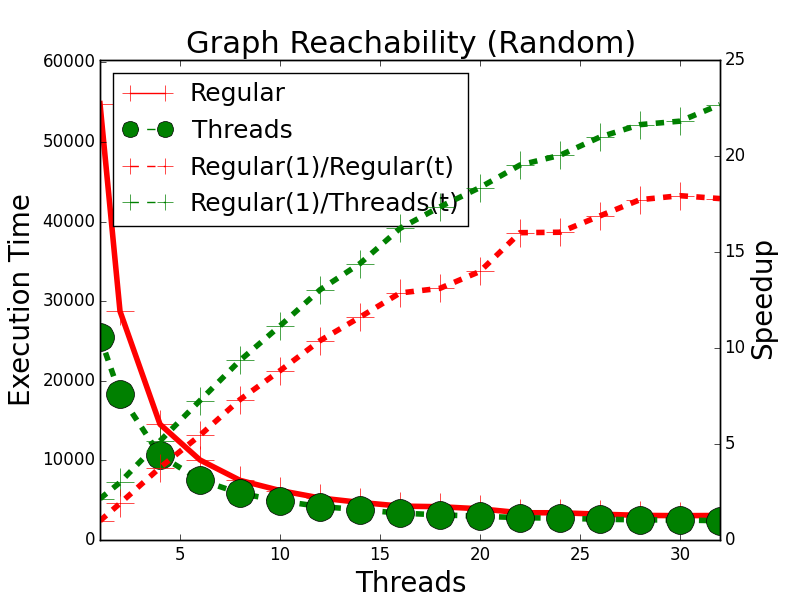
\includegraphics[width=\textwidth]{experiments/threads/cmp-search-random.png}
           \caption{Random is a graph with 50000 nodes and 1052674
              edges. The dataset makes 20 graph queries
              to 5\% of the graph's nodes.}
           \label{fig:threads:search_random}
        \end{subfigure}
        \spacing
        \begin{subfigure}[b]{\plotsize\textwidth}
           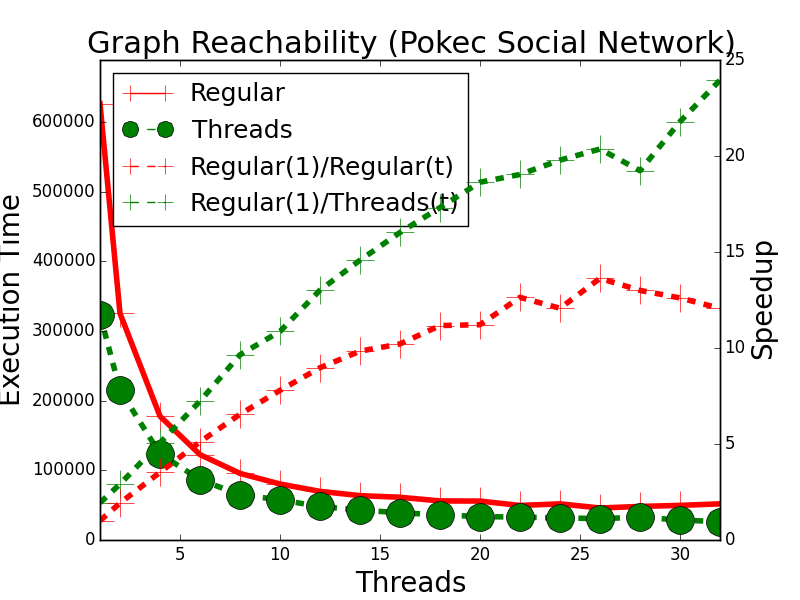
\includegraphics[width=\textwidth]{experiments/threads/cmp-search-pokec.png}
           \caption{Pokec has 1632803 nodes and 30622564 edges. The dataset
           makes 3 graph queries to 1\% of the graph's nodes.}
           \label{fig:threads:search_pokec}
        \end{subfigure} \\
        \caption{Measuring the performance of the graph reachability program
        when using thread facts.}
        \label{fig:threads:results_search}
\end{figure}

The graph reachability program shows how to introduce complex coordination
policies between threads by reasoning about the state of each thread. In
addition, the use of linear logic programming makes it easier to prove
properties of the program since computation is done by applying controlled
changes to the state.


\clearpage
